\chapter{Heterogeneidade em estados de equilíbrio}
\label{cap.Heterogeneidade}

\section{Introdução}

O conceito de heterogeneidade de tamanhos de domínios foi inicialmente introduzido no contexto de um modelo de grafo aleatório~\cite{LeeKimPark}, construído através da introdução de uma modificação no modelo de Erdős-Rényi~\cite{Achlioptas}. O modelo de Erdős-Rényi descreve um particular processo de construção de um grafo aleatório: inicia-se com $N$ vértices isolados e adicionam-se ligações entre os mesmos, uma a cada passo, através da escolha aleatória de dois vértices. Com a sucessiva adição de novas ligações, surgem domínios de vértices conectados. A heterogeneidade de tamanhos de domínios é definida como o número de tamanhos distintos de domínios existentes em determinada configuração de um sistema, sendo o tamanho de um domínio dado pelo número de vértices contidos no mesmo.

Definindo como um parâmetro de controle do sistema uma densidade de ligações $t \equiv K/N$, sendo $K$ o número de ligações, verifica-se que para um determinado valor $t_c$, o modelo apresenta uma transição de fase, denominada transição de percolação, caracterizada pelo aparecimento de um domínio de dimensões macroscópicas (componente gigante), definido como um domínio que escala com $N$. Definindo-se um parâmetro de ordem $g(t) \equiv G(t)/N$, onde $G(t)$ é o tamanho do maior domínio, verifica-se que no limite $N \rightarrow \infty$, para $t < t_c$ temos $g(t)=0$, enquanto que para $t > t_c$, $g(t)$ tem um valor finito, evidenciando a presença de duas fases distintas, sendo a transição entre uma fase e outra contínua.

O modelo descrito na Ref.~\cite{Achlioptas} define um método alternativo para a construção do grafo: partindo-se de $N$ vértices isolados, a cada passo escolhe-se aleatoriamente dois pares de vértices, escolhendo-se então, entre os dois pares, para a construção de uma nova ligação, aquele que minimiza o produto dos tamanhos dos domínios a serem conectados. O modelo baseado nessa \textit{regra do produto} atraiu considerável interesse, por exibir uma transição de fase aparentemente descontínua, diferentemente do que é encontrado no modelo de Erdős-Rényi e outros modelos de percolação, tendo sido denominado este comportamento de percolação explosiva. O caráter contínuo ou descontínuo da transição foi elucidado no trabalho de Lee \textit{et al}~\cite{LeeKimPark}, onde foi demonstrado que, assim como as transições observadas nos modelos mais tradicionais de percolação, a transição na percolação explosiva era também contínua. A figura \ref{fig.ErdosProduct} ilustra o processo de construção de um grafo de acordo com os modelos de Erdős-Rényi e da regra do produto.

\begin{figure}
 \centering
 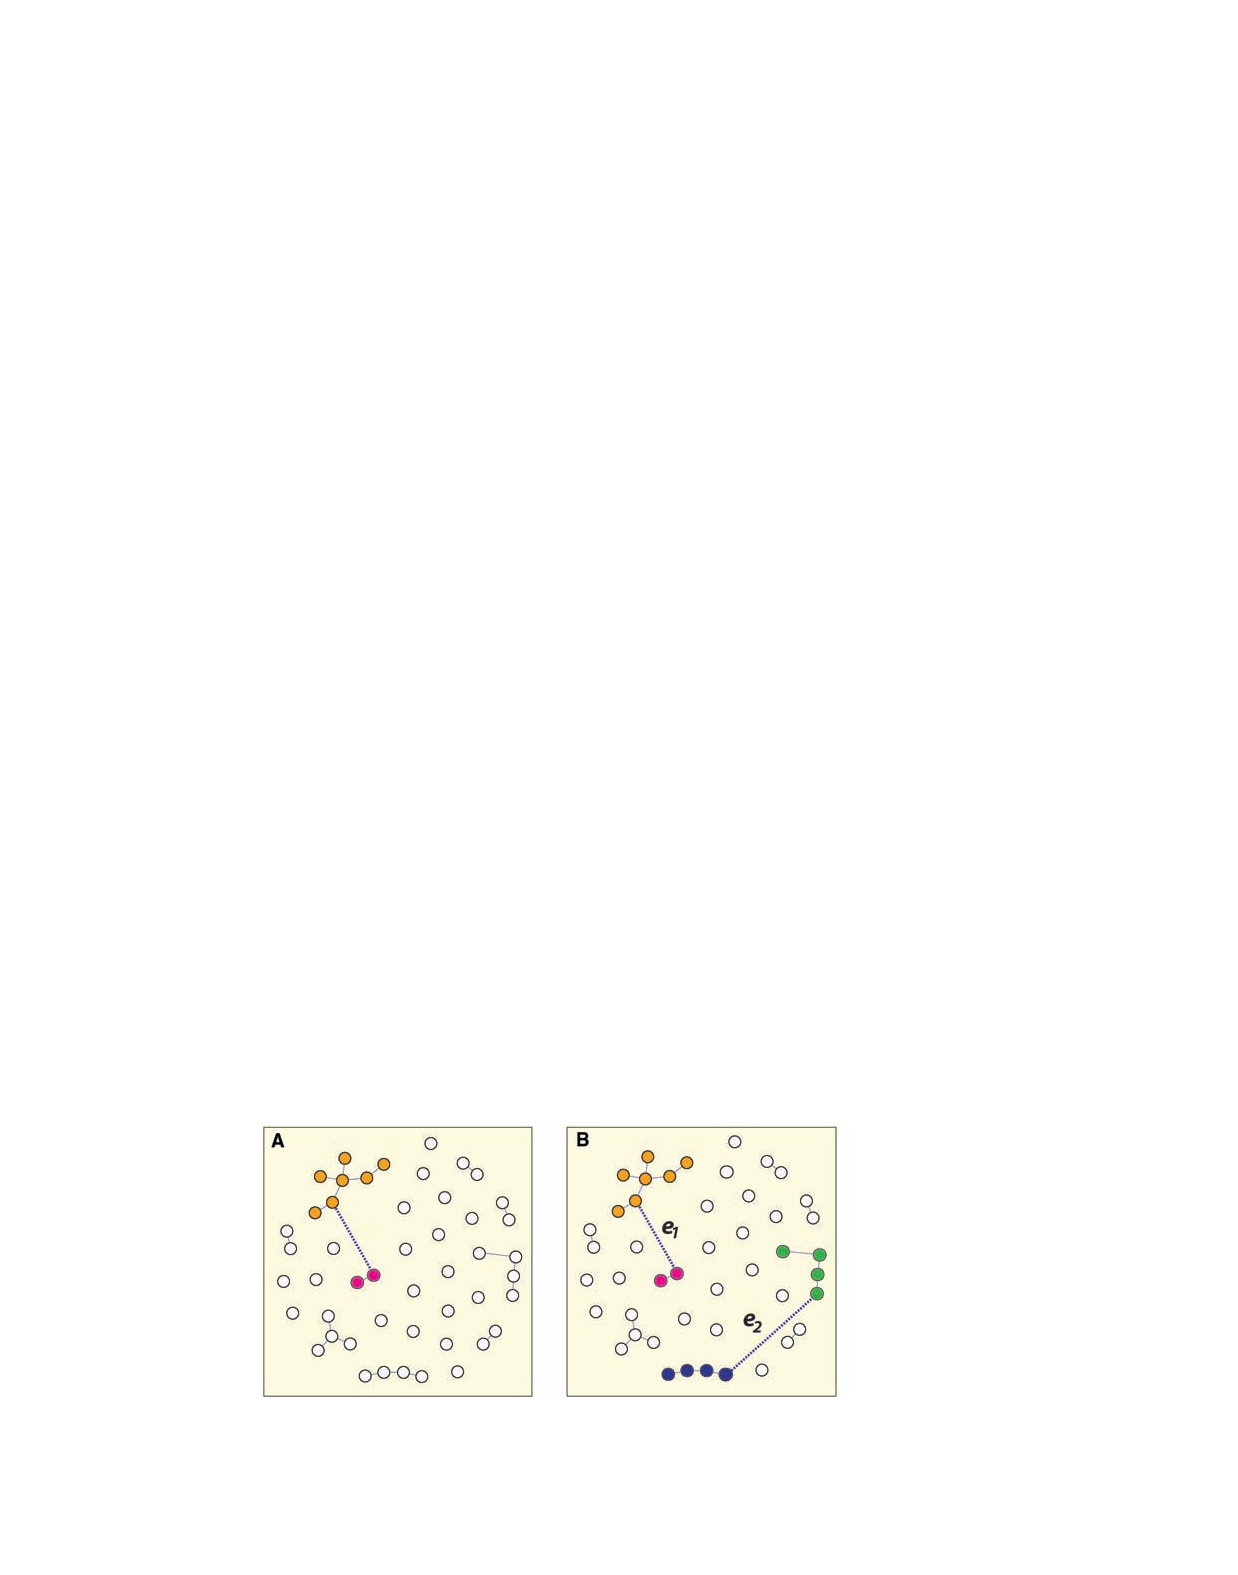
\includegraphics[width=14cm]{img/ErdosProduct.pdf}
 \caption{Processo de construção do grafo. (A) no modelo de Erdős-Rényi, a cada passo, dois vértices são selecionados aleatoriamente e conectados por uma nova ligação. (B) em modelos que incorporam um determinado grau de escolha, a cada passo, dois pares de vértices são selecionados aleatoriamente e um dos pares é escolhido de acordo com alguma regra, como a regra do produto, e então conectado por uma nova ligação, enquanto que o outro par é desconsiderado~\cite{Achlioptas}.}
\label{fig.ErdosProduct}
\end{figure}

O argumento descrito por Lee \textit{et al} utiliza dois pseudo-pontos de transição, $t_l$ e $t_u$, definidos respectivamente como limites inferior e superior para o real ponto de transição $t_c$, convergindo assintoticamente ao mesmo no limite $N \rightarrow \infty$. O ponto $t_l$ foi definido como o ponto em que se observa um máximo na heterogeneidade dos tamanhos de domínios de vértices conectados. No estado inicial do grafo, existe apenas um tamanho de domínio (domínios formados por vértices isolados). Com a adição de novas ligações, e consequente aumento do parâmetro de controle $t$, vão surgindo outros tamanhos de domínios no sistema, e a medida de heterogeneidade aumenta. Entretanto, a partir de determinado ponto, aparece um domínio de dimensões macroscópicas que começa a absorver domínios menores, levando a uma progressiva redução da heterogeneidade, até que, eventualmente, exista um único domínio contendo todos os vértices. Como a regra do produto torna desfavorável o aparecimento de domínios grandes, espera-se que a heterogeneidade aumente lentamente, mas constantemente, com o aumento de $t$, até um ponto imediatamente antes do ponto $t_c$, em que domínios de diferentes tamanhos são combinados em um grande domínio~\cite{LeeKimPark}. O ponto $t_u$ foi definido como o ponto imediatamente subsequente ao ponto em que o tamanho do segundo maior domínio tem seu valor máximo. Os autores utilizaram simulações numéricas para validar as hipóteses acerca do comportamento dos pontos $t_l$ e $t_u$. A figura \ref{fig.tltu} mostra a variação dos valores de $t_l$ e $t_u$ com o aumento de $N$.

\begin{figure}
 \centering
 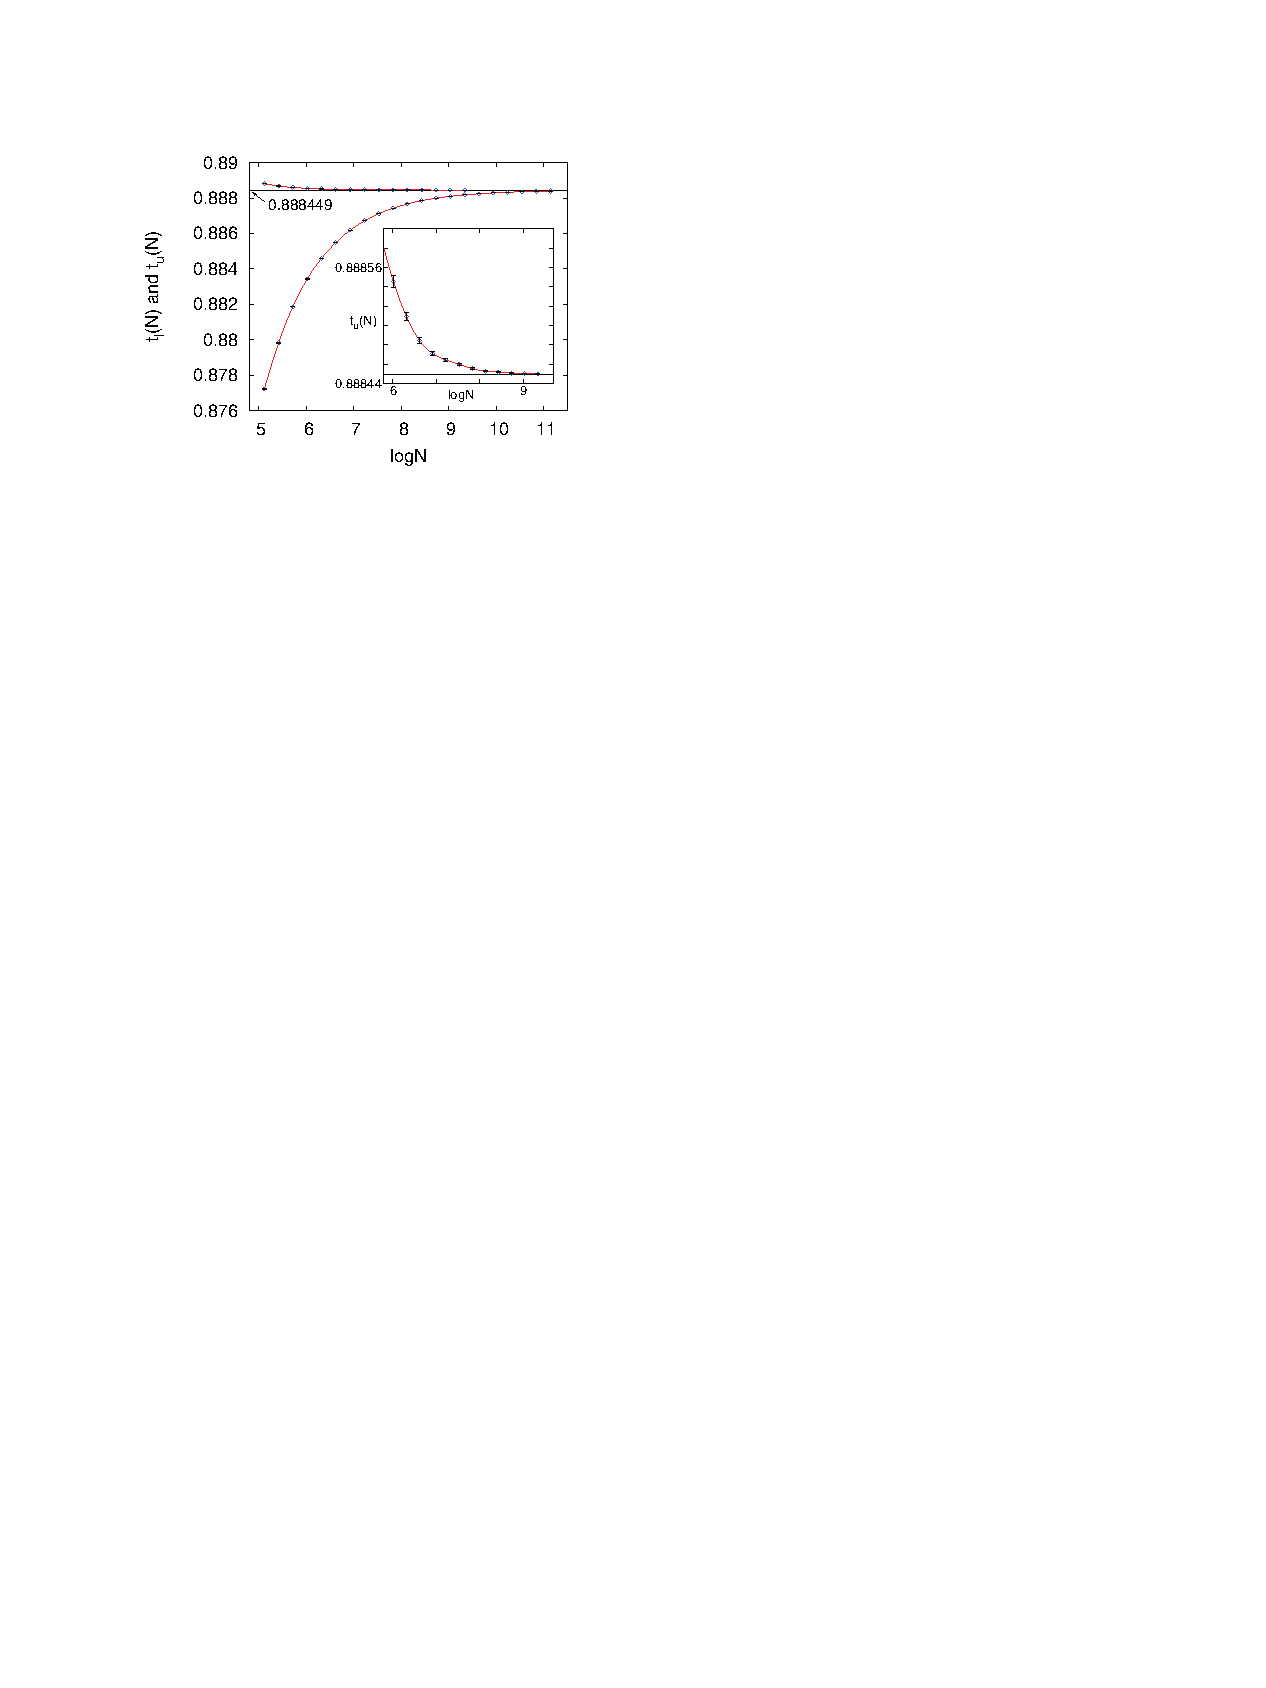
\includegraphics[width=14cm]{img/tltu.pdf}
 \caption{Variação de $t_l$ (ramo inferior) e $t_u$ (ramo superior) com o tamanho do sistema. No limite termodinâmico, $t_l$ e $t_u$ convergem para o valor de $t_c = 0.8884490(5)$~\cite{LeeKimPark}.}
\label{fig.tltu}
\end{figure}

A Ref.~\cite{LeeKimPark} utiliza a definição de $t_l$ e $t_u$ em um argumento que não será detalhado aqui, determinando um limite superior para o aumento de tamanho sofrido pelo maior domínio entre os pontos $t_l$ e $t_u$, verificando que esse aumento é sub-linear em $N$, o que implica a inexistência de um salto finito no valor do parâmetro de ordem na transição de fase, no limite $N \rightarrow \infty$, refutando assim a hipótese de uma transição descontínua na percolação explosiva. 

O sucesso do uso da heterogeneidade de tamanhos de domínios no modelo de percolação explosiva motivou o estudo detalhado das propriedades dessa medida, bem como a sua aplicação a outros modelos, como modelos de percolação de ligações e de sítios~\cite{NohLeePark}, definidos sobre uma rede, assim como os modelos de Ising~~\cite{JoYiBaekKim} e de Potts~\cite{LvYangDeng}.


\section{Heterogeneidade em modelos de percolação de rede}

Dois dos mais estudados modelos de percolação são o modelo de percolação de ligações e o modelo de percolação de sítios, definidos sobre uma rede com determinada geometria. No primeiro, ligações são estabelecidas entre primeiros-vizinhos na rede com uma probabilidade $p$. As ligações definem domínios de sítios conectados. Já no modelo de percolação de sítios, os sítios da rede estão ocupados com uma probabilidade $p$, ou vazios com probabilidade $1-p$, sendo que sítios ocupados adjacentes (primeiros vizinhos) são considerados como pertencentes a um mesmo domínio. Em ambos os modelos, a partir de determinado valor crítico $p_c$ da probabilidade $p$, também chamado de limiar de percolação, aparece um domínio macroscópico, definido da mesma forma que para o modelo de Erdős-Rényi. Define-se o parâmetro de ordem $m$ como a fração dos sítios pertencentes ao domínio macroscópico.

Noh \textit{et al}~\cite{NohLeePark} estudaram a heterogeneidade de tamanhos de domínios nos modelos de percolação de sítios e de ligações, utilizando escalamento de tamanhos finitos (\textit{finite size scaling} - FSS), verificando que a mesma satisfaz a equação:
\begin{equation}
 \label{eq.HetPerc}
 H(\epsilon,L) = L^{d/\tau} f(|\epsilon| L^{1/\nu_H}),
\end{equation} 
onde $\epsilon \equiv p-p_c$, $L$ é o tamanho linear da rede, $d$ é o número de dimensões, $\tau$ é o chamado expoente de Fisher, que caracteriza a distribuição de tamanhos de domínios, $f$ é a função de escala associada à heterogeneidade, e $\nu_H$ é um novo expoente crítico. Para justificar essa lei de escala, Noh \textit{et al}~\cite{NohLeePark} e Jo \textit{et al}~\cite{JoYiBaekKim} apresentam o seguinte argumento. Embora a distribuição de tamanhos de domínios não seja em geral conhecida exatamente (uma exceção é quando $p=p_c$), a sua forma segue
\begin{equation}
n(A) \sim A^{-\tau} \exp(-A/A_c),
\end{equation}
onde\footnote{Cabe notar que o $\tau$ aqui utilizado corresponde ao $\tau^\prime$ definido na seção~\ref{sec.DistAreasDomGeo}.} $\tau=187/91$ e $A_c$ é o tamanho característico dos domínios. Devido ao termo exponencial, $A_c$ funciona como um parâmetro de corte (\textit{cutoff}) para a distribuição: somente os domínios com $A<A_c$ aparecem em número significativo e a distribuição, até esse ponto, segue a lei de potência $A^{-\tau}$. À medida que o sistema se aproxima do limiar de percolação, $A_c$ diverge e ficamos somente com a lei de potência. Isto define um expoente crítico $\sigma$, $A_c \sim |\epsilon|^{-1/\sigma}$. Portanto, se o sistema estiver longe do limiar crítico, a heterogeneidade coincidirá com $A_c$,
$$
H \sim A_c \sim |\epsilon|^{-1/\sigma},
$$ 
pois domínios com $A>A_c$ serão raros\footnote{$n(A)$, qualquer que seja, é proporcional ao número de domínios com tamanho $A$, portanto $\int_0^{A_c}n(A)dA$ será proporcional ao número total de domínios. Para contar apenas uma vez o tamanho $A$, devemos dividir o integrando por $n(A)$. Então temos: $H \sim \int_0^{A_c}\frac{n(A)}{n(A)}dA = A_c$.}. Por outro lado, na região crítica ($|\epsilon|\ll 1$), o tamanho linear do sistema, $L$, se torna importante pois é ele que limita o tamanho máximo que os domínios podem ter. Após uma região com comportamento tipo lei de potência, a distribuição de áreas passa a ter um pico antes de cair abruptamente. Aproximadamente até a posição deste pico os domínios aparecem com uma probabilidade significativa. Então podemos definir uma quantidade $A_n$ (próxima à posição do pico), tal que $A_n$ é a maior área para a qual, dentre os $N_c$ domínios existentes no sistema, ainda temos, em média, pelo menos um deles com esta área. Assim, $n(A_n) \sim 1/N_c$ e, estatisticamente, não teremos áreas maiores do que $A_n$. Portanto, 
$$
H\sim A_n, |\epsilon|\ll 1.
$$
Como $n(A_n) \sim A_n^{-\tau}$, temos $A_n \sim N_c^{1/\tau}$. Além disso, nesta região, $N_c$ é comparável ao tamanho total da rede, $N=L^d$, logo $A_n \sim L^{d/\tau}$. Assim temos:
\begin{equation}
H(\epsilon,L) \sim \left\{
\begin{array}{l}
L^{d/\tau}, \text{ na região crítica } (|\epsilon|\ll 1) \\
|\epsilon|^{-1/\sigma}, \text{ longe da região crítica.}
\end{array}
\right. 
\end{equation} 

Esses dois comportamentos limites podem ser descritos por uma lei de escala do tipo da Eq.~(\ref{eq.HetPerc}), onde $\nu_H=\tau/d\sigma$ e a função de escala satisfaz $f(x)\sim cte$ quando $x\ll 1$ e $f(x)\sim x^{-1/\sigma}$, caso contrário.

A figura \ref{fig.HetPerc} mostra a variação da heterogeneidade com o parâmetro $p$, para modelos de percolação de sítios e de ligações, em redes bidimensionais quadradas e triangulares, utilizando dados obtidos a partir de simulações baseadas no método de Monte Carlo. A figura \ref{fig.HetPercCol} mostra o colapso dos mesmos dados, de acordo com a forma da Eq.~(\ref{eq.HetPerc}).

\begin{figure}
 \centering
 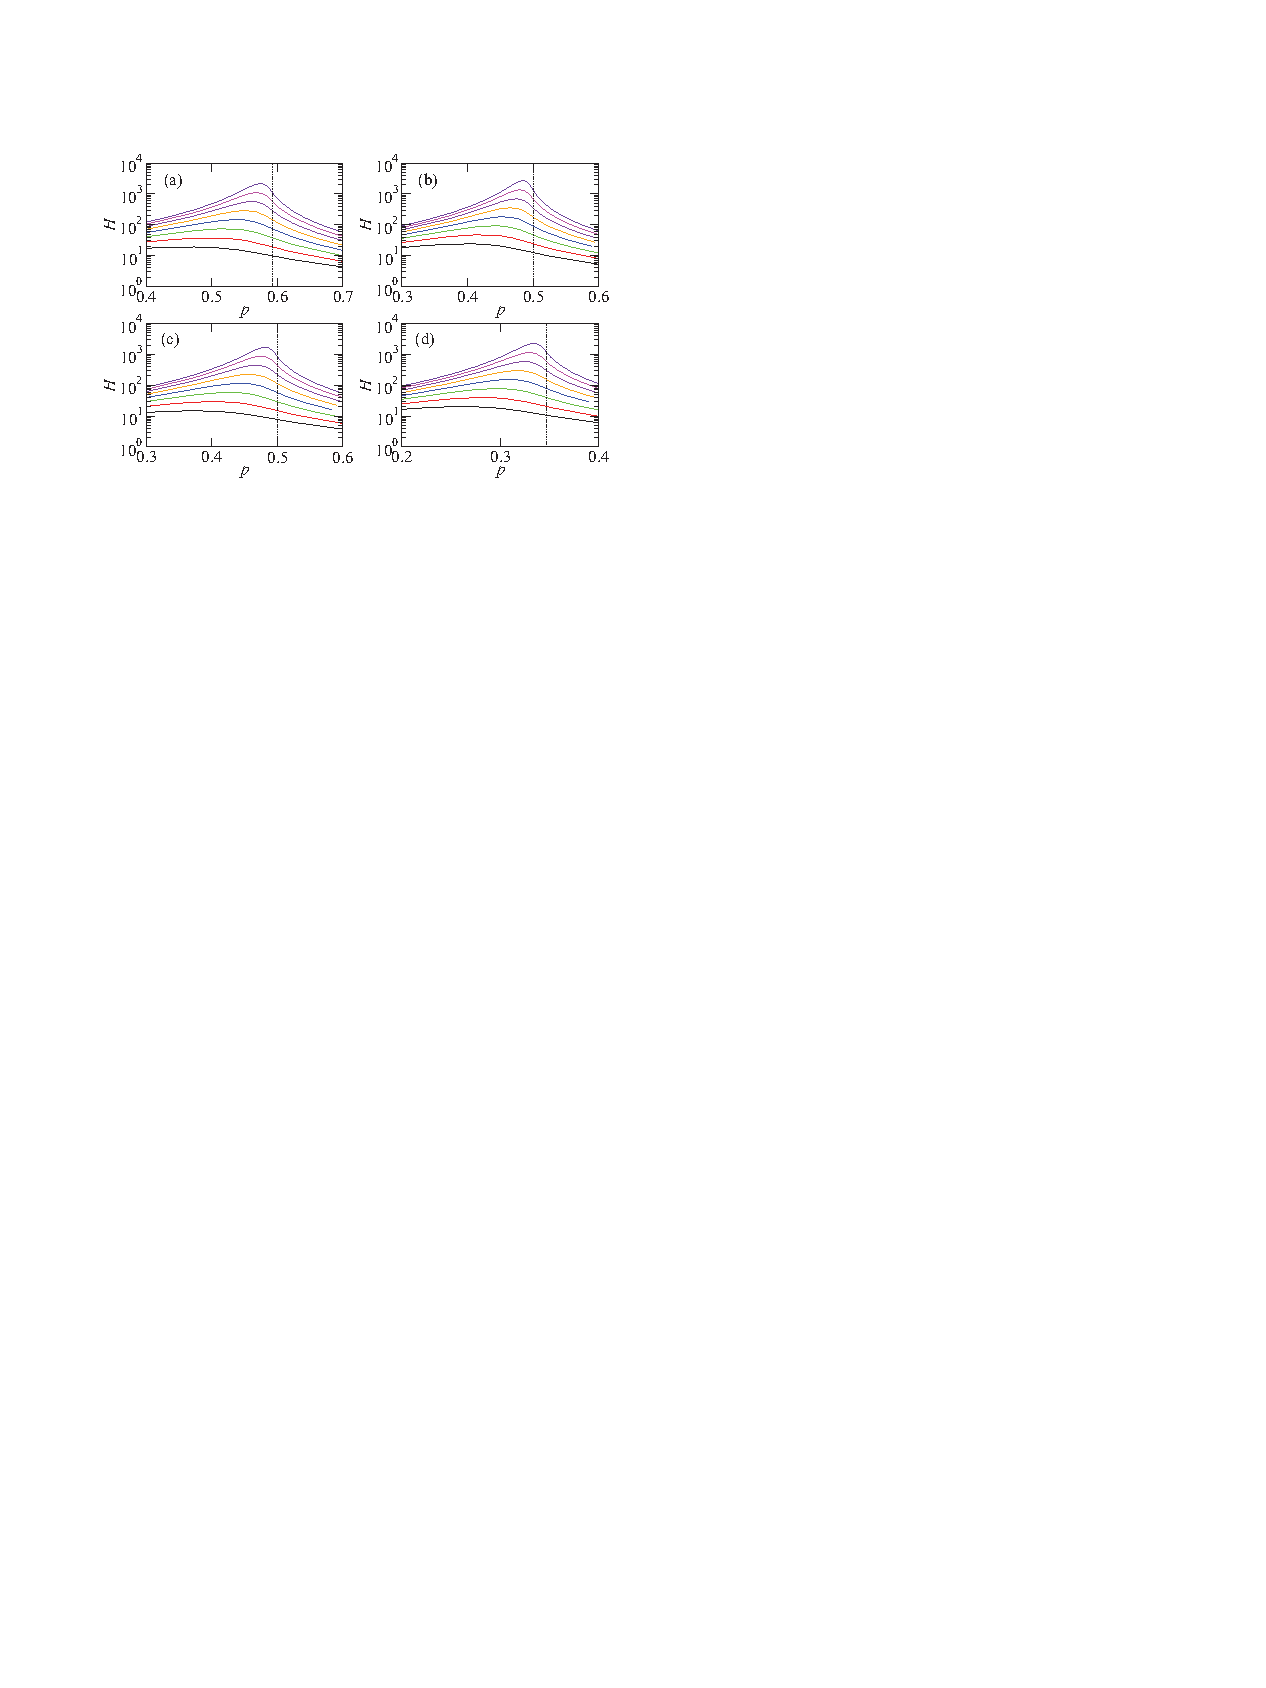
\includegraphics[width=14cm]{img/HetPerc.pdf}
 \caption{Variação da heterogeneidade de tamanhos de domínios em modelos de percolação de sítios em (a) e (c) e de ligações em (b) e (d), na rede quadrada em (a) e (b), e na rede triangular em (c) e (d). A linha pontilhada representa o limiar de percolação. Os tamanhos de rede são $L=2^5, \ldots, 2^{12}$ para a rede quadrada e $L=27 \times 2^0, \ldots, 27 \times 2^7$ para a rede triangular. Quanto maior o valor de $L$, mais alto o valor de $H$~\cite{NohLeePark}.}
\label{fig.HetPerc}
\vspace{8mm}
 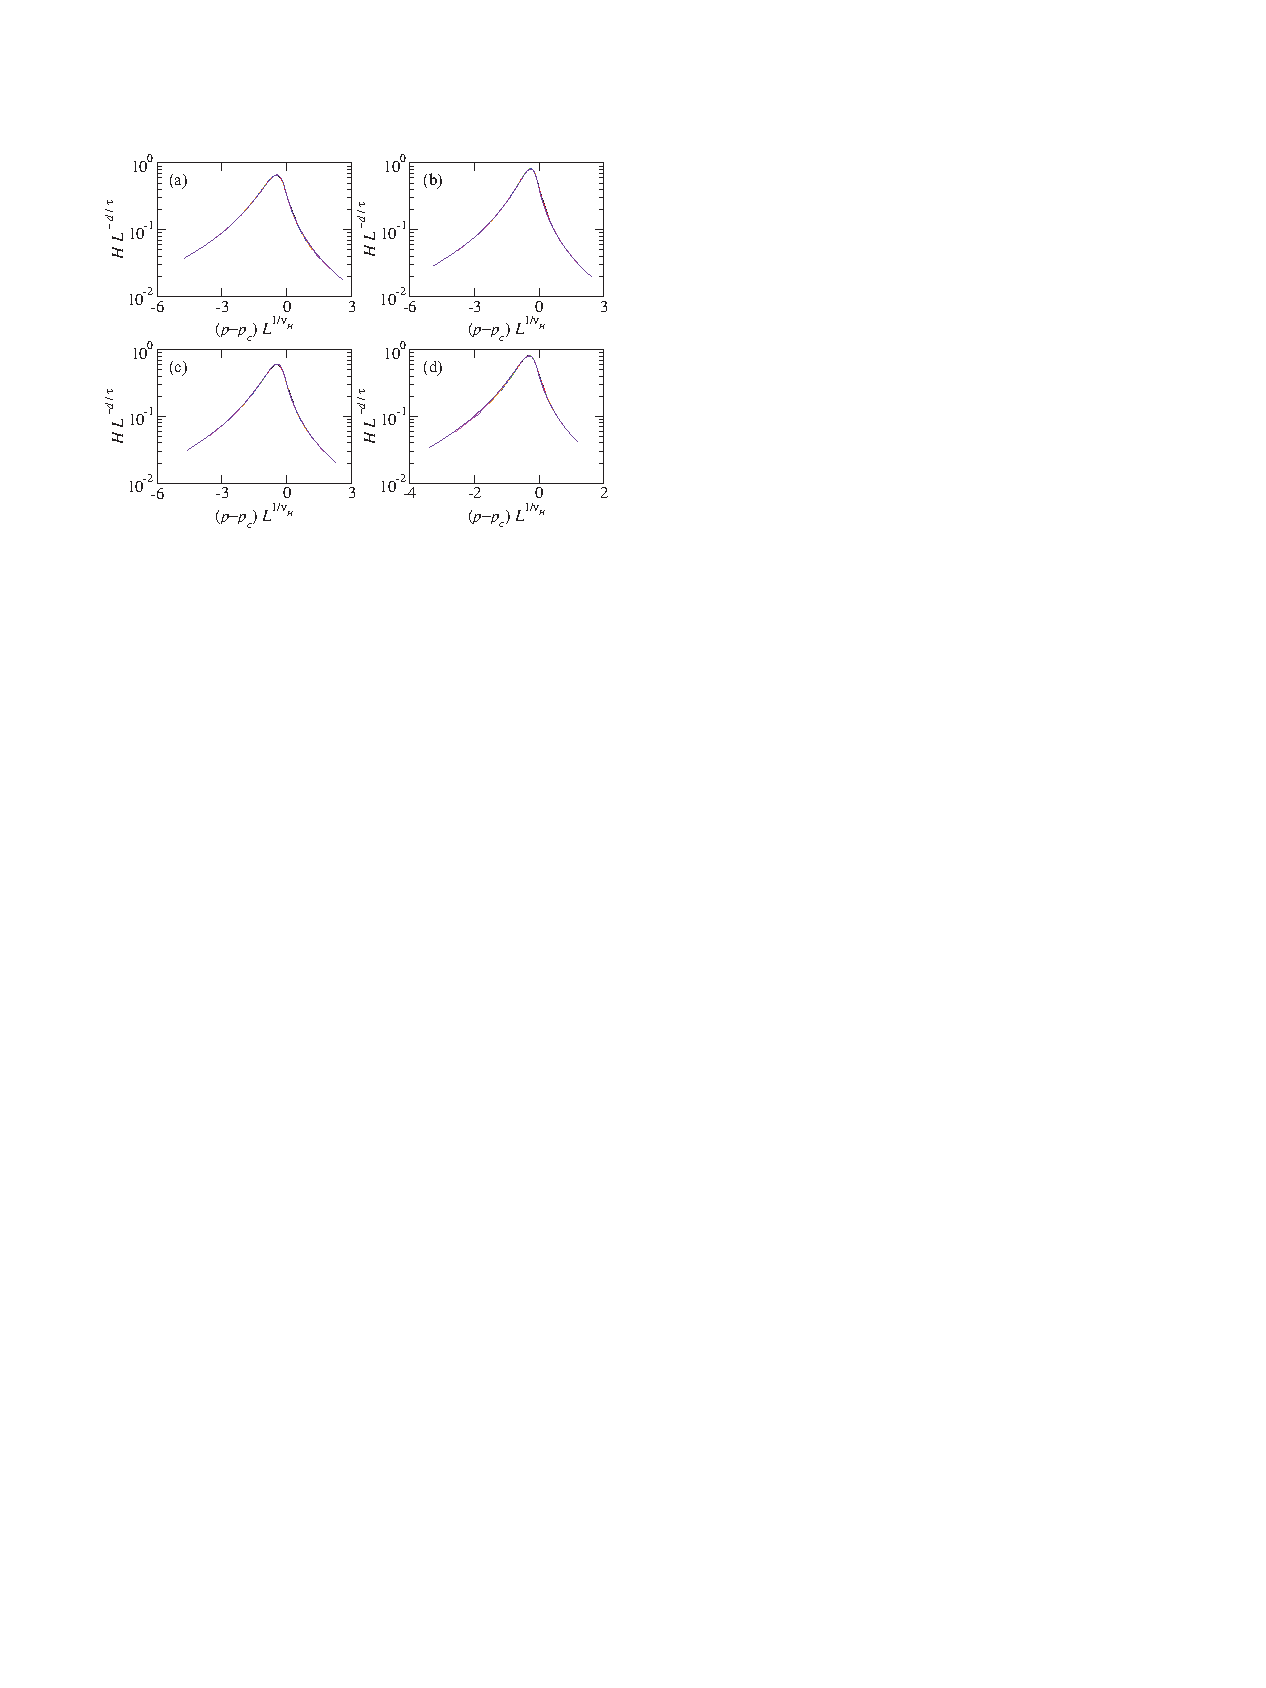
\includegraphics[width=14cm]{img/HetPercCol.pdf}
 \caption{Análise de escala da heterogeneidade de tamanhos de domínios em modelos de percolação de sítios em (a) e (c) e de ligações em (b) e (d), na rede quadrada em (a) e (b), e na rede triangular em (c) e (d). Os dados são os mesmos utilizados na figura \ref{fig.HetPerc}~\cite{NohLeePark}.}
\label{fig.HetPercCol}
\end{figure}


\section{Heterogeneidade no modelo de Ising}

Jo \textit{et al}~\cite{JoYiBaekKim} estudaram a heterogeneidade de tamanhos de domínios geométricos no modelo de Ising em duas dimensões, verificando a validade da forma de escala dada pela Eq.~(\ref{eq.HetPerc}), com a troca do parâmetro $\epsilon$ por $t \equiv (T-T_c)/T_c$, e determinando numericamente o valor do expoente $\nu_H$, através de simulações de Monte Carlo, obtendo um resultado em excelente concordância com o valor $\nu_H = 379/192$, determinado analiticamente com base em expoentes obtidos via teoria de campo conforme (\textit{conformal field theory} - CFT). A figura \ref{fig.IsingH} mostra a variação da heterogeneidade de tamanhos de domínios geométricos no modelo de Ising em duas dimensões, em uma rede quadrada, para estados de equilíbrio, com a variação da temperatura, para vários tamanhos de rede, com dados obtidos através de simulações de Monte Carlo. A figura~\ref{fig.IsingHCol} mostra o colapso dos mesmos dados, de acordo com a forma da Eq.~(\ref{eq.HetPerc}) e do valor obtido para o expoente $\nu_H$.

\begin{figure}
 \centering
 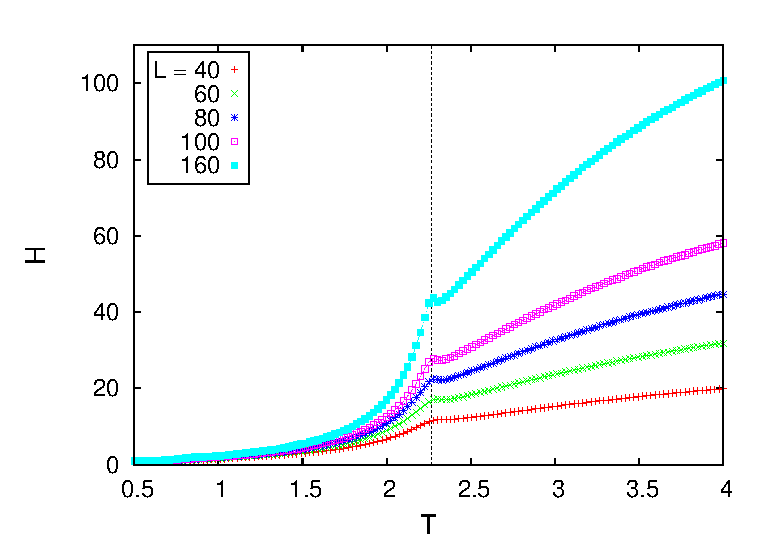
\includegraphics[width=14cm]{fig/hetequi_q2.eps}
 \caption{Heterogeneidade de tamanhos de domínios geométricos no modelo de Ising em duas dimensões, na rede quadrada, em estados de equilíbrio, em função da temperatura, para diversos tamanhos de rede. A linha pontilhada indica a temperatura crítica $T_c$.}
\label{fig.IsingH}
\vspace{8mm}
 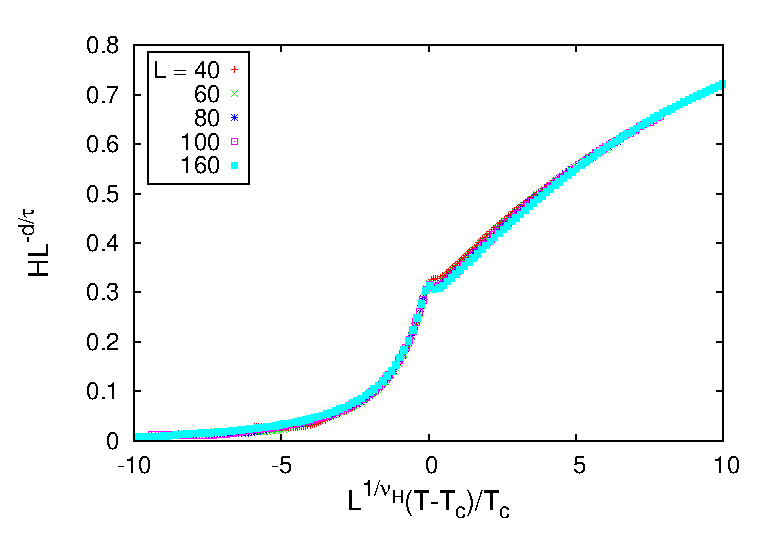
\includegraphics[width=14cm]{fig/hetequi_q2_colXY.eps}
 \caption{Análise de escala da heterogeneidade de tamanhos de domínios geométricos no modelo de Ising em duas dimensões, na rede quadrada, em estados de equilíbrio, em função da temperatura. Os dados são os mesmos utilizados na figura \ref{fig.IsingH}.}
\label{fig.IsingHCol}
\end{figure}

